\documentclass[tikz,border=10pt]{standalone}
\usepackage{tikz}
\usepackage{amsmath}

\begin{document}
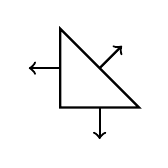
\begin{tikzpicture}
    % Define the vertices of the reference triangle
    \coordinate (A) at (0,0);
    \coordinate (B) at (1,0);
    \coordinate (C) at (0,1);

    % Draw the triangle
    \draw[black, thick] (A) -- (B) -- (C) -- cycle;

    % Label the vertices
%    \node[below left] at (A) {$A$};
%    \node[below right] at (B) {$B$};
%    \node[above left] at (C) {$C$};

    % Draw vector fields with arrows
	\draw[->, black, thick] (0.5, 0) -- (0.5, -0.4);   
	\draw[->, black, thick] (0.5, 0.5) -- (0.783,0.783);   
	\draw[->, black, thick] (0, 0.5) -- (-0.4, 0.5);  

    % Local coordinate system within the triangle
%    \node at (1.5,1) {$\mathbf{u}(x,y) = \begin{pmatrix} a + bx \\ c + dy \end{pmatrix}$};

\end{tikzpicture}
\end{document}



